\documentclass[dvipdfmx,11pt,notheorems]{beamer}
%%%% 和文用 %%%%%
\usepackage{bxdpx-beamer}
\usepackage{pxjahyper}
\usepackage{minijs}%和文用
\usepackage{listings,jlisting} % プログラムの表示用
\usepackage{type1cm}
\renewcommand{\kanjifamilydefault}{\gtdefault}%和文用

%%%% tikz 用 %%%%%
\usepackage[latin1]{inputenc}
\usepackage{tikz}
\usetikzlibrary{intersections}
\usetikzlibrary{shapes,arrows}

%%%% スライドの見た目 %%%%%
\usetheme{Boadilla}
\usecolortheme{seahorse}
\usefonttheme{professionalfonts}
\setbeamertemplate{frametitle}[default][center]
\setbeamertemplate{navigation symbols}{}
\setbeamercovered{transparent}%好みに応じてどうぞ)
\setbeamertemplate{footline}[page number]
\setbeamerfont{footline}{size=\normalsize,series=\bfseries}
\setbeamercolor{footline}{fg=black,bg=black}

\setbeamercolor{white-cyan1}
{fg=white,bg=cyan!80!black}
\setbeamercolor{white-cyan2}
{fg=white,bg=cyan!60!black}

%フラットデザイン化
\setbeamertemplate{blocks}[rounded] % Blockの影を消す
%Beamer色設定
\definecolor{UniBlue}{RGB}{0,150,200}
\definecolor{AlertOrange}{RGB}{255,76,0}
\definecolor{AlmostBlack}{RGB}{38,38,38}
\setbeamercolor{structure}{fg=UniBlue} % 見出しカラー
\setbeamercolor{block title}{fg=UniBlue!50!black} % ブロック部分タイトルカラー
%%%%

%%%% 定義環境 %%%%%
\usepackage{amsmath,amssymb}
\usepackage{amsthm}
\usepackage{bm}
\theoremstyle{definition}
\newtheorem{theorem}{定理}
\newtheorem{definition}{定義}
\newtheorem{proposition}{命題}
\newtheorem{lemma}{補題}
\newtheorem{corollary}{系}
\newtheorem{conjecture}{予想}
\newtheorem*{remark}{Remark}
\renewcommand{\proofname}{}
% 定義
\DeclareMathOperator*{\argmin}{arg\,min}
\DeclareMathOperator*{\argmax}{arg\,max}
\def\vec#1{\mbox{\boldmath$#1$}}
\def\R{{\Bbb R}}
%%%%%%%%%

%%%%% フォント基本設定 %%%%%
% \usepackage[T1]{fontenc}%8bit フォント
% \usepackage{textcomp}%欧文フォントの追加
% \usepackage[utf8]{inputenc}%文字コードをUTF-8
% \usepackage{otf}%otfパッケージ
% \usepackage{lxfonts}%数式・英文ローマン体を Lxfont にする
% \usepackage{bm}%数式太字
%%%%%%%%%%

%%%%% 複数人の著者を揃える %%%%%
%% http://tex.stackexchange.com/questions/
%%   166531/how-to-change-author-alignment-in-beamer
\makeatletter
\long\def\beamer@author[#1]#2{%
  \def\insertauthor{\def\inst{\beamer@insttitle}\def\and{\beamer@andtitle}%
  \begin{tabular}{rl}#2\end{tabular}}%
  \def\beamer@shortauthor{#1}%
  \ifbeamer@autopdfinfo%
    \def\beamer@andstripped{}%
    \beamer@stripands#1 \and\relax
    {\let\inst=\@gobble\let\thanks=\@gobble\def\and{, }\hypersetup{pdfauthor={\beamer@andstripped}}}
  \fi%
}
\makeatother
%%%%%%%%%%

%%%%% プログラムに色をつける
\usepackage{color}

\definecolor{codegreen}{rgb}{0,0.6,0}
\definecolor{codegray}{rgb}{0.5,0.5,0.5}
\definecolor{codepurple}{rgb}{0.58,0,0.82}
\definecolor{backcolour}{rgb}{0.95,0.95,0.92}

\lstdefinestyle{mystyle}{
    backgroundcolor=\color{backcolour},
    commentstyle=\color{codegreen},
    keywordstyle=\color{magenta},
    numberstyle=\tiny\color{codegray},
    stringstyle=\color{codepurple},
    basicstyle=\footnotesize,
    breakatwhitespace=false,
    breaklines=true,
    captionpos=b,
    keepspaces=true,
    numbers=left,
    numbersep=5pt,
    showspaces=false,
    showstringspaces=false,
    showtabs=false,
    tabsize=2
}

\lstset{style=mystyle}

%%%%
\title[略タイトル]{第4回 知能システム学特論レポート}%[略タイトル]{タイトル}
\author[NishidaLab]{
15344203 & 有田 裕太 \\
15344206 & 緒形 裕太 \\
15344209 & 株丹 亮 \\
12104125 & 宮本 和 }%[略名前]{名前}
\institute[NishidaLab]{西田研究室,計算力学研究室}%[略所属]{所属}
\date{2015年\ 6月\ 29日}%日付

\begin{document}

%%%% 1 %%%%
\begin{frame}[plain]\frametitle{}
\titlepage %表紙
\end{frame}

% \begin{frame}\frametitle{Contents}
% \tableofcontents %目次
% \end{frame}

\section{進捗状況}
%%%% 2 %%%%
\begin{frame}\frametitle{進捗状況}

\begin{block}{理論研究の進捗}
人工ニューラルネットワークの理論について
\end{block}

\vspace{1cm}
\begin{exampleblock}{プログラミングの進捗}
なし
\end{exampleblock}
\end{frame}

%%%% 3.1.1 %%%%
\begin{frame}[fragile]\frametitle{ユニットの出力}

\begin{figure}[tb]
  \begin{center}
    
\includegraphics[clip,width=4cm]{fig/eps/input_output.eps}
  \end{center}
  \caption{ユニット1つの入出力の例}
\end{figure}

\begin{itemize}
\item 各ユニットは複数の入力を受けて1つの出力を計算する.
\item 各入力に対しそれぞれ異なる重み$w1$,$w2$,$w3$,$w4$を入力$x1$,$x2$,$x3$,$x4$に掛けたものの和にバイアス値$b$を加える.
\end{itemize}

\end{frame}

%%%% 3.1.2 %%%%
\begin{frame}[fragile]\frametitle{ユニットの出力}

\begin{block}{総入力$u$とユニットの出力$z$}
\begin{eqnarray}
  u & = & w_1x_1+w_2x_2+w_3x_3+w_4x_4+b\\
  z & = & f(u)
\end{eqnarray}
\end{block}
これを一般化し\\
第1層のユニットを$i=1,\cdots,I$,第2層のユニットを$j=1,\cdots,J$で表すと
\begin{block}{入出力式の一般化}
\begin{eqnarray}
  u_j & = & \sum_{i=1}^I w_{ji}x_i + b_j\\
  z_j & = & f(u_j)
\end{eqnarray}
\end{block}
\end{frame}


%%%% 3.2.1 %%%%
\begin{frame}[fragile]\frametitle{活性化(シグモイド)関数}

\begin{figure}[tb]
  \begin{center}
    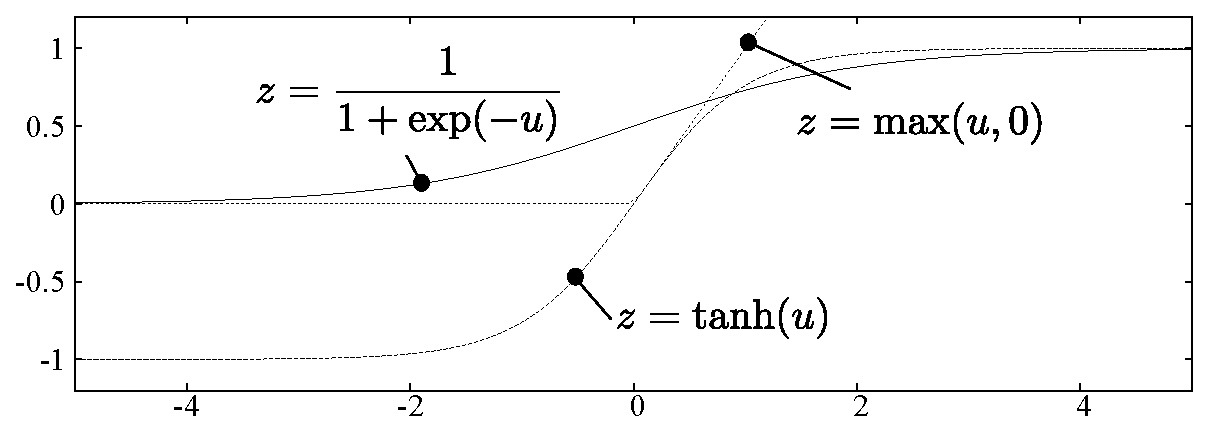
\includegraphics[clip,width=9cm]{fig/eps/sigmoid.eps}
  \end{center}
  \caption{典型的なシグモイド関数}
\end{figure}
\end{frame}

%%%% 3.2.2 %%%%

\begin{frame}[fragile]\frametitle{マックスアウト}

\begin{block}{マックスアウト関数}
\begin{align}
 u_{jk}=\sum w_{jik}z_i +b_{jk}\ \ (1...K)\\
 f(u_{j})=\max_{k=1...K}(u_{jk})
\end{align}
\vspace{0.1mm}
\end{block}

\begin{itemize}
\item ユニットをまとめたような構造を持つ.
\item 異なる重みとバイアスを持つそれぞれの総入力を別々に計算し\\
最大値をユニットの出力とする.
\end{itemize}
\end{frame}


%%%% 3.3.1 %%%%
\begin{frame}[fragile]\frametitle{多層ネットワーク}

\begin{figure}[tb]
  \begin{center}
    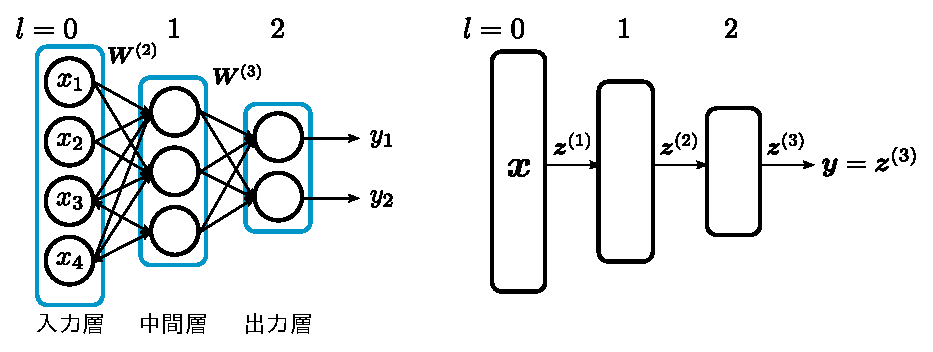
\includegraphics[clip,width=9cm]{fig/eps/unit.eps}
  \end{center}
  \caption{2層のネットワーク}
\end{figure}

\begin{itemize}
\item 入力$\bm{u}^{(l)}$,出力$\bm{z}^{(l)}$
\item 各層間の結合重み$\bm{W}^{(l)}\ (l=2,\cdots, L)$
\item ユニットのバイアス$\bm{b}^{(l)}\ (l=2,\cdots, L)$
\end{itemize}

\end{frame}

%%%% 3.3.2 %%%%
\begin{frame}[fragile]\frametitle{多層ネットワーク}

\begin{figure}[tb]
  \begin{center}
    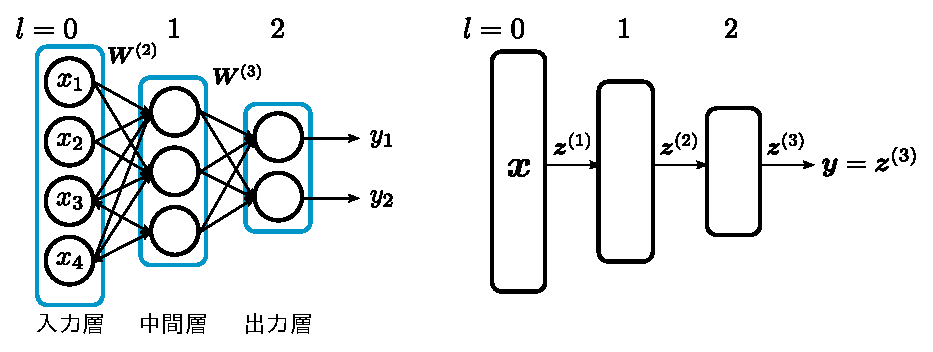
\includegraphics[clip,width=9cm]{fig/eps/unit.eps}
  \end{center}
  \caption{2層のネットワーク}
\end{figure}
中間層($l=2$),出力層($l=3$)はそれぞれ
\begin{eqnarray}
\label{eq:3a}
  \bm{u}^{(2)} &=& \bm{W}^{(2)}\bm{x} + \bm{b}^{(2)} \nonumber\\
  \bm{z}^{(2)} &=& \bm{f}(\bm{u}^{(2)}) \nonumber\\
  \bm{u}^{(3)} &=& \bm{W}^{(3)}\bm{z}^{(2)} + \bm{b}^{(3)} \nonumber\\
  \bm{z}^{(3)} &=& \bm{f}(\bm{u}^{(3)})\nonumber
\end{eqnarray}
\end{frame}

%%%% 3.3.3 %%%%

\begin{frame}[fragile]\frametitle{多層ネットワーク}

\begin{block}{任意の階層 L のネットワークに一般化すると}
\begin{eqnarray}
  \bm{u}^{(l+1)} &=& \bm{W}^{(l+1)}\bm{z}^{(l)} + \bm{b}^{(l+1)} \\
  \bm{z}^{(l+1)} &=& \bm{f}(\bm{u}^{(l+1)})
\end{eqnarray}
\vspace{0.1mm}
\end{block}

\begin{itemize}
\item $l=1,\ 2,\ 3,\cdots, L-1$の順に繰り返していくと最終的な出力$\bm{y}$を決定することができる.
\item 各層間の結合重み$\bm{W}^{(l)}$とユニットのバイアス$\bm{b}^{(l)}$を成分に持つベクトル$\bm{w}$を定義する.\\
\item これを$\bm{y}(\bm{x};\bm{w})$と表現する.
\end{itemize}
\end{frame}

%%%% 3.4 %%%%
%%%% 3.4.1 %%%%

\begin{frame}[fragile]\frametitle{出力層の設計と誤差関数}

順伝播型ネットワークが表現する関数$\vec{y}(\vec{x};\vec{w})$をネットワークのパラメータ$\vec{w}$を変えることで変化させ,望みの関数を与える.
\begin{eqnarray}
 \{(\vec{x}_{1},\mathrm{d}_{1}),(\vec{x}_{1},\mathrm{d}_{1}),...,(\vec{x}_{N},\mathrm{d}_{N})\}
\end{eqnarray}
これらのペア$(\vec{x},\mathrm{d})$1つ1つを訓練サンプル(training samples)といい,その集合を訓練データ(training data)という.
学習とはネットワーク$\vec{w}$を調整することで訓練データの入出力ペアをで
 きるだけ再現すること.

ネットワークが表す関数と訓練データとの近さ$(\vec{y}(\vec{x}_{n};\vec{w}))$を誤差関数(error function)で定義する.誤差関数は問題の種別や活性化関数によって異なる.

\begin{table}[htb]
\centering
\caption{問題の種別ごとの活性化関数と誤差関数}
\label{000718_27Jun15}
\begin{tabular}[bt]{|c|c|c|}\hline
 問題の種別& 出力層の活性化関数&誤差関数 \\ \hline \hline
 回帰&正接双曲線関数や恒等写像 & 二乗誤差 式\eqref{000645_27Jun15}\\
 二値分類& ロジスティック関数& 式\eqref{000654_27Jun15}\\
 多クラス分類& ソフトマックス関数& 交差エントロピー 式\eqref{000700_27Jun15}\\ \hline
\end{tabular}
\end{table}
\end{frame}

%%%% 3.4.2 %%%%
\begin{frame}[fragile]\frametitle{回帰}
\begin{block}{回帰}
出力連続値をとる関数を対象に訓練データを良く再現する関数を求めることをいう.回帰では活性化関数に正接双曲線関数や恒等写像を用いる
\end{block}
\begin{exampleblock}{評価関数}
\begin{eqnarray}
 E(\vec{w}) = \displaystyle{\frac{1}{2}}\sum^{N}_{n=1}||\vec{d}_{n}-\vec{y}(\vec{x}_{n};\vec{w})||^{2}\label{000645_27Jun15}
\end{eqnarray}
\vspace{0.1cm}
\end{exampleblock}
\end{frame}

%%%% 3.4.3 %%%%
\begin{frame}[fragile]\frametitle{二値分類}
\begin{block}{二値分類}
入力$\vec{x}$に応じて2種類に区別する問題を考える.すなわち,$d\in\{0,1\}$とする.このとき,活性化関数はロジスティック関数$y=1/(1+\exp(-u))$とする.
\end{block}
\begin{exampleblock}{評価関数}
\begin{eqnarray}
E(\vec{w})=-\sum^{N}_{n=1}\left[d_{n}\log y(\vec{x}_{n};\vec{w} + (1-d_{n})\log\{1-y(\vec{x}_{n};\vec{w})\})\right]\label{000654_27Jun15}
\end{eqnarray}
\vspace{0.1cm}
\end{exampleblock}
\end{frame}

%%%% 3.4.4 %%%%
\begin{frame}[fragile]\frametitle{多クラス分類}
\begin{block}{多クラス分類}
入力$\vec{x}$に応じて有限個のクラスに分類する問題である.活性化関数にはソフトマックス関数(softmax function)が良く用いられる.
\end{block}
\begin{exampleblock}{活性化関数と評価関数}
\begin{eqnarray}
 y_{k} \equiv z_{k}^{(L)}= \frac{\exp(u_{k}^{(L)})}{\sum^{K}_{j=1}exp(u_{j}^{(L)})} \\
E(\vec{w})=-\sum^{N}_{n=1}\sum^{N}_{k=1}d_{nk}\log y_{k}(\vec{x}_{n};\vec{w})\label{000700_27Jun15}
\end{eqnarray}
\vspace{0.1cm}
\end{exampleblock}

\end{frame}

%%%% 5 %%%%
\begin{frame}\frametitle{今後の課題}

\begin{block}{理論研究}
DNN,CNN,caffeについて理解を深める
\end{block}

\vspace{1cm}
\begin{exampleblock}{プログラミング}
中間層の出力,可視化
\end{exampleblock}
\end{frame}

% \begin{figure}[t]
%  \begin{minipage}{0.3\hsize}
%   \centering
%   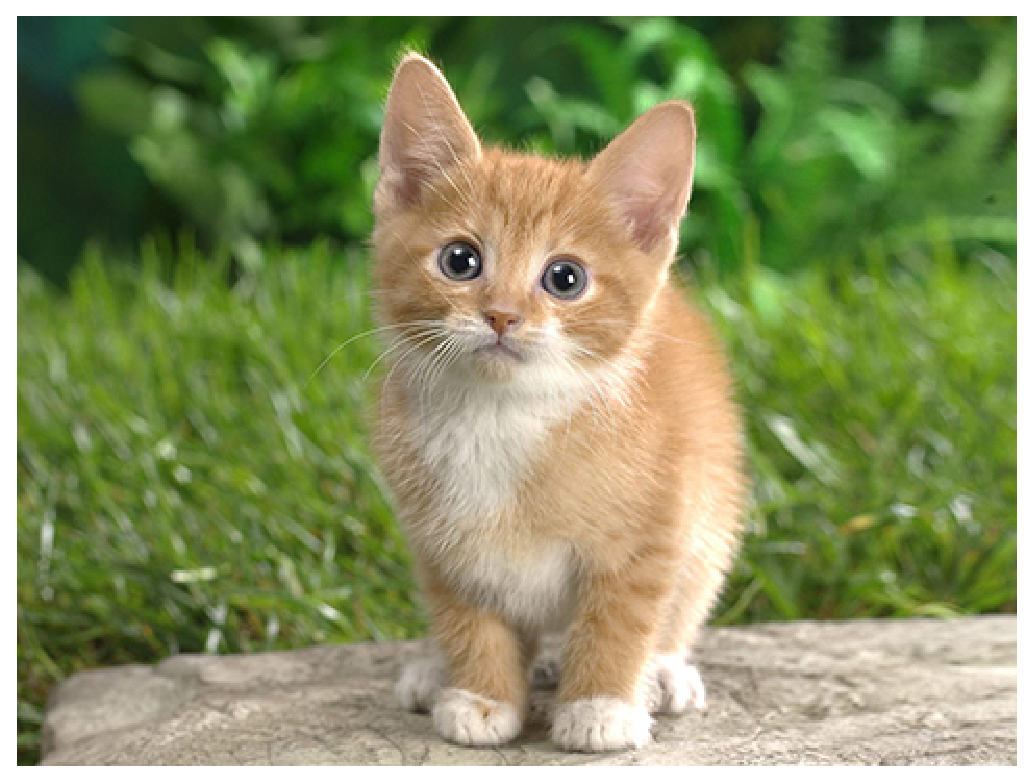
\includegraphics[width=30mm]{./figure/cat.eps}
%   \caption{cat.jpg}
%   \label{sample1}
%  \end{minipage}
%  \begin{minipage}{0.3\hsize}
%   \centering
%   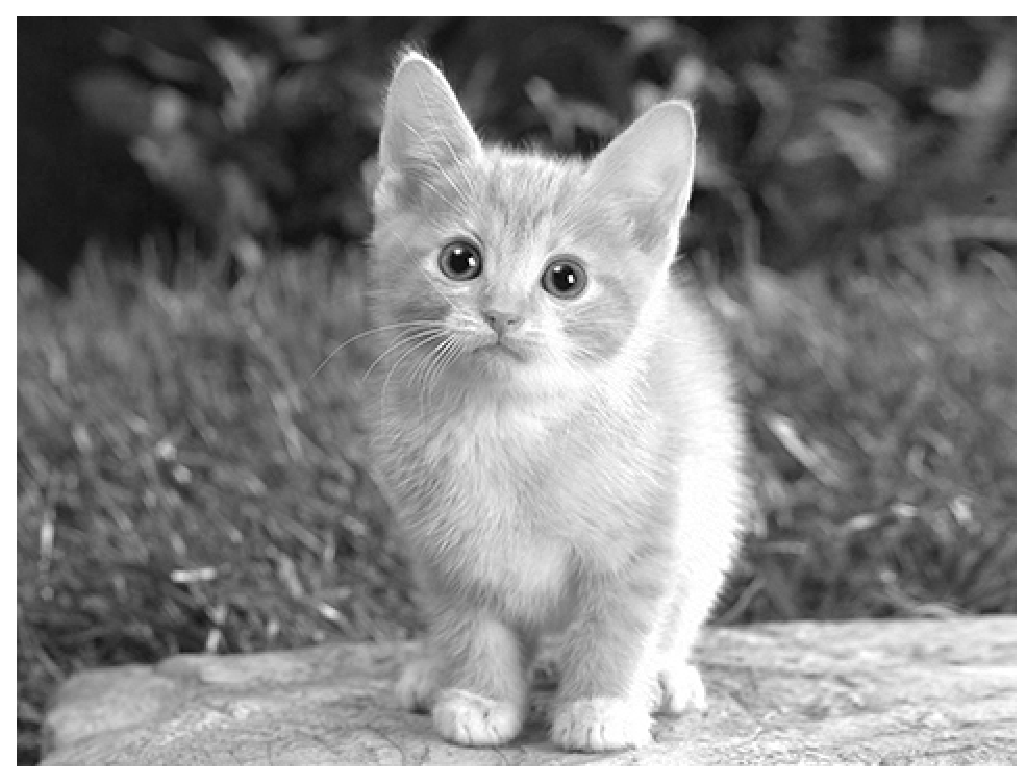
\includegraphics[width=30mm]{./figure/cat_gray.eps}
%   \caption{cat\_gray.jpg}
%   \label{sample2}
%  \end{minipage}
%  \begin{minipage}{0.3\hsize}
%   \centering
%   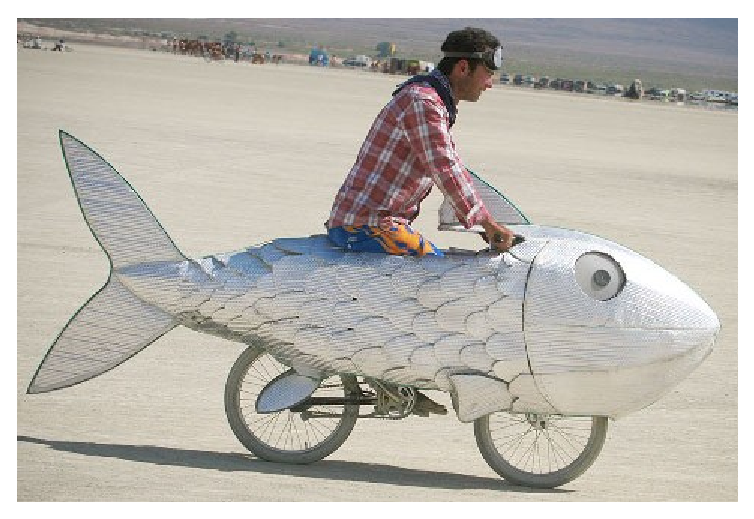
\includegraphics[width=30mm]{./figure/fish-bike.eps}
%   \caption{fish-bike.jpg}
%   \label{sample3}
%  \end{minipage}
% \end{figure}
% \begin{exampleblock}{実行環境}
% \begin{itemize}
%  \item Ubuntu 14.04 LTS
%  \item Intel core i5-4440 3.10GHz$\times$4
%  \item RAM 16GB
% \end{itemize}
% \end{exampleblock}
% \end{frame}


% \section{具体例}

% \begin{frame}\frametitle{定理環境の例}
% \begin{theorem}[Fermat]
% $a^{p-1} \equiv 1 \pmod{p}$
% \end{theorem}
% \pause
% \begin{theorem}[Wilson]
% \begin{equation}
% (p-1)! \equiv 1 \pmod{p}
% \end{equation}
% \end{theorem}
% \end{frame}

% \begin{frame}<1-2>\frametitle{オーバーレイ}
% \onslide*<1>{
% \Large{これは1枚目です}
% }
% \onslide*<2>{
% これは2枚目です
% \begin{theorem}[Euclid]
% There is no largest prime number.
% \end{theorem}
% }
% \end{frame}

% \begin{frame}\frametitle{色もつけれるよ}
%   {\color{red} red}(\alert{alert}),
%   {\color{blue} blue}(\structure{structure}),
%   {\color{green} green},
%   {\color{cyan} cyan},
%   {\color{magenta} magenta},
%   {\color{yellow} yellow},
%   {\color{black} black},
%   {\color{darkgray} darkgray},
%   {\color{gray} gray},
%   {\color{lightgray} lightgray},
%   {\color{orange} orange},
%   {\color{violet} violet},
%   {\color{purple} purple},
%   {\color{brown} brown},
% \end{frame}

% \begin{frame}\frametitle{いろんなブロック}
% \begin{block}{ブロック}
% これは普通のブロックです
% \end{block}

% \begin{alertblock}{警告ブロック}
% 警告!これは警告ブロックだ!
% \end{alertblock}

% \begin{exampleblock}{例ブロック}
% 例えば、こんなブロックです。
% \end{exampleblock}
% \end{frame}

% \begin{frame}<1-2>\frametitle{画像も貼れるよ}
% \onslide*<1>{
% このように画像を貼れるよ
% %\begin{figure}[htb]
% %\centering
% %\includegraphics[width=12cm,clip]{dummygraph.pdf}
% %\caption{$f(x)=e^{-\frac{x}{10}}\sin(x)$}
% %\end{figure}%
% }
% \onslide*<2>{
% 画像や表は各自用意してね
% %\begin{figure}[htb]
% %\centering
% %\includegraphics[width=8cm,clip]{sym4.pdf}
% %\caption{Cayley graph of $\mathfrak{S}_{4}$}
% %\end{figure}%
% }
% \end{frame}

% \begin{frame}\frametitle{まとめ}
% \LARGE{大事なのは中身です!}
% \end{frame}

% \begin{frame}\frametitle{}
% {\Large ありがとうございました}
% \end{frame}
% \appendix

\newcounter{finalframe}
\setcounter{finalframe}{\value{framenumber}}

% \begin{frame}[containsverbatim]\frametitle{dvipngの使い方(1)}
% \begin{block}{この様なファイルを用意する}
% \tiny{
% \begin{verbatim*}
% \documentclass[43pt]{jsarticle}
% \usepackage{amsmath}
% \usepackage{lmodern}
% \pagestyle{empty}
% \begin{document}
% \begin{equation*}
% \sum_{k=0}^{\infty} \frac{(2k)!}{2^{2k}(k!)^2} \frac{1}{2k+1}=\frac{\pi}{2}
% \end{equation*}
% \end{document}
% \end{verbatim*}
% }
% \end{block}
% \end{frame}

% \begin{frame}[containsverbatim]\frametitle{dvipngの使い方(2)}
% \begin{block}{使い方(コマンドライン)}
% \scriptsize{
% \begin{verbatim*}
% latex dvipng-sample.tex
% dvipng dvipng-sample.dvi -T tight -bd 1000
% \end{verbatim*}
% }
% \end{block}
% \end{frame}
\setcounter{framenumber}{\value{finalframe}}
\end{document}